% !TeX root = construct.tex

\chapter{Steiner's Straight-edge Problem}\label{c.chapter}

\begin{quote}
This document is Problem $34$ from the book by Heinrich D\"{o}rrie: \textit{100 Problems of Elementary Mathematics: Their History and Solution} (Dover, 1965), as reworked by Michael Woltermann.\footnote{\url{http://www2.washjeff.edu/users/mwoltermann/Dorrie/DorrieContents.htm}. I would like to thank him for giving me permission to use his work.} I have added explanations so that students and teachers can better understand the construction. The document has been written and formatted in \LaTeX{}, and I have redrawn the diagrams using Ti\textit{k}Z, adding auxiliary lines and  drawing diagrams incrementally for clarity.

Moti Ben-Ari\footnote{\url{http://www.weizmann.ac.il/sci-tea/benari/}.}\\
Department of Science Teaching\\
Weizmann Institute of Science
\end{quote}

\bigskip

\textbf{Prove that every construction that can be done with compass and straight-edge can be done with straight-edge alone given a fixed circle in the plane.}

As far back as 1759 Lambert had solved a whole series of geometric constructions with straight-edge alone in his book \textit{Freie Perspektive}, published in Z\"{u}rich that year. He is also the source of the term ``straight-edge geometry''. After Lambert, French mathematicians, primarily Poncelet and Brianchon, took up straight-edge geometry, particularly after the publication of Mascheroni's \textit{Geometria del compasso} gave a new stimulus to these studies, and they attempted to find as many constructions as possible with straight-edge alone. 

With a straight-edge alone, it is possible to represent only rational algebraic expressions (so not for example, $\sqrt{ab}$).
\begin{quote}
In the nineteenth century it was shown that any length constructed with a straight-edge and compass can be obtained from a given unit length by the operations of rational arithmetic ($+,-,\times,\div$) together with the operation of computing square roots. This was used to prove that it is impossible to trisect an angle or double a cube, because they require the construction of a length that is a cube root. The sentence above explains the reason why a straight-edge alone is not sufficient to perform all constructions. 
\end{quote}

This suggested to Poncelet that an additional fixed circle (with its center) must be given in order to draw with straight-edge alone all algebraic expressions that can be constructed with compass and straight-edge. This was confirmed by Jakob Steiner (1796-1863), the greatest geometer since the days of Appolonius, in his celebrated book \textit{Die geometrischen Konstruktionen asgef\"{u}hrt mittels der geraden Linie und Eines festen Kreises} (Geometrical constructions carried out with straight lines and a fixed circle), Berlin, 1833. 

The solution presented here is based on that in Steiner's book, except that we have eliminated everything that is not strictly essential for the purpose at hand, and we have also made it somewhat more elementary. Since in straight-edge geometry, the intersection of two straight lines is known directly, we need only demonstrate that the two fundamental problems II and III of No. 33 can be solved using a straight-edge and fixed circle. 
\begin{quote}
From Problem 33: When we examine the separate steps by which circle and straight-edge constructions are carried out, we see that every step consists of one of the following three basic constructions:

I. Finding the point of intersection of two straight lines;

II. finding the point(s) of intersection of a straight line and a circle;

III. finding the point(s) of intersection of two circles.

The following notation from Problem 33 is used here:
\begin{itemize}
\item $c(O,A)$ stands for the circle with center $O$ through point $A$,
\item $c(O,AB)$ stands for the circle with center $O$ and radius $AB$.
\end{itemize}
What does it mean to perform a construction with straight-edge alone? A circle is defined by a point $O$ (its center) and a line segment (whose length is the radius $r$) one of whose endpoints is the center. The following diagram shows what it means to determine $X,Y$, the points of intersection of a line and a circle, and of two circles. Since we don't have a compass, the dashed lines in the diagram don't actually appear in the construction. Similarly, any circle in the diagrams of this document only help understand a construction and its proof.
\begin{center}
\begin{tikzpicture}[scale=.9]
\fill (0,0) node[above right] {$O$} circle[radius=2pt];
\draw[thick,dashed,name path=circle] (0,0) circle[radius=2cm];
\draw (0,0) -- node[left] {$r$} ++(-60:2cm);
\fill (0,0) ++(-60:2cm) circle[radius=2pt];
\draw[name path=line] (-3,-.5) -- ++(20:6cm);
\path [name intersections={of=circle and line,by={X,Y}}];
\fill (X) node[above right,xshift=-2pt,yshift=4pt] {$X$} circle[radius=2pt];
\fill (Y) node[above left] {$Y$} circle[radius=2pt];
\begin{scope}[xshift=6cm]
\fill (0,0) node[above right] {$O_1$} circle[radius=2pt];
\fill (3,0) node[above right] {$O_2$} circle[radius=2pt];
\draw[thick,dashed,name path=circle1] (0,0) circle[radius=2cm];
\draw[thick,dashed,name path=circle2] (3,0) circle[radius=2cm];
\draw (0,0) -- node[left] {$r_1$} ++(-60:2cm);
\draw (3,0) -- node[left,below] {$r_2$} ++(-20:2cm);
\fill (3,0) ++(-20:2cm) circle[radius=2pt];
\path [name intersections={of=circle1 and circle2,by={X,Y}}];
\fill (X) node[above,yshift=4pt] {$X$} circle[radius=2pt];
\fill (Y) node[below,yshift=-4pt] {$Y$} circle[radius=2pt];
\end{scope}
\end{tikzpicture}
\end{center}
\end{quote}
As in the solution of Mascheroni's problem, we must first solve several preliminary problems, in this case five of them. 

\textbf{Prelim 1.} Construct a line through point $P$ parallel to a given line. ($P$ is not on the given line.)

\textbf{Solution.} Steiner considers two cases: 
\begin{itemize}
\item \textbf{1a.} two points $A$ and B and their midpoint M on the given line are known. We will call the straight line a "directed straight line" in this case.
\item \textbf{1b.} the given straight line is arbitrary. 
\end{itemize}

\textbf{1a.} Draw $AP$ and let $S$ be a point on $AP$ extended. Connect $S$ with $M$ and $B$. Let $O$ be the intersection point of $BP$ and $MS$. Finally let line $AO$ meet $BS$ at $Q$.

\begin{center}
\vspace*{-8pt}
\begin{tikzpicture}
\draw[name path=pq] (-4,0) -- (4,0);
\draw (-2,-2) node[below left] {$A$} coordinate (A) -- (2,-2) node[below right] {$B$} coordinate (B);
\fill (A) circle[radius=2pt];
\fill (B) circle[radius=2pt];
\draw[name path=as] (A) -- ++(50:4cm) node[above] {$S$} coordinate (S);
\fill (S) circle[radius=2pt];
\draw[name path=sb] (S) -- (B);
\path [name intersections={of=pq and as,by={P}}];
\path [name intersections={of=pq and sb,by={Q}}];
\fill (P) node[above left] {$P$} circle[radius=2pt];
\fill (Q) node[above right] {$Q$} circle[radius=2pt];
\draw[name path=pb] (P) -- (B);
\draw[name path=qa] (Q) -- (A);
\path [name intersections={of=pb and qa,by={O}}];
\fill (O) node[right,xshift=2pt] {$O$} circle[radius=2pt];
\fill (0,-2) coordinate (M) node[below right] {$M$} circle[radius=2pt];
\draw (S) -- (M);
\end{tikzpicture}
\vspace*{-6pt}
\end{center}
\begin{quote}
Note the order in which the lines are constructed. The line segment $AB$ and its midpoint $M$ are given, as is $P$, the point through which the parallel line is to be drawn. $S$ is an arbitrary point on the extension of $AP$. Once $S$ is chosen, the lines $SB$ and $SM$ can be constructed. Then $BP$ is constructed and its intersection with $SM$ is defined to be $O$. Next, a ray is from $A$ through $O$ intersects $SB$ at $Q$ and the line $PQ$ is constructed. It appears from the diagram that $PQ$ is parallel to $AB$, but that is precisely what has to be proved.
\end{quote}
By Ceva's Theorem,
\[
\frac{AM}{MB}\frac{BQ}{QS}\frac{SP}{PA} = 1
\]
\begin{quote}
To prove Ceva' Theorem, examine the following diagrams.
\begin{center}
\vspace*{-8pt}
\begin{tikzpicture}
\path[name path=pq] (-4,0) -- (4,0);
\draw (-2,-2) node[below left] {$A$} coordinate (A) -- (2,-2) node[below right] {$B$} coordinate (B);
\coordinate (M) at (0,-2);
\draw[name path=as] (A) -- ++(50:4cm) node[above] {$S$} coordinate (S);
\draw[name path=sb] (S) -- (B);
\path [name intersections={of=pq and as,by={P}}];
\path [name intersections={of=pq and sb,by={Q}}];
\path[name path=pb] (P) -- (B);
\path[name path=qa] (Q) -- (A);
\path [name intersections={of=pb and qa,by={O}}];
\draw[fill=gray!40] (B) -- (O) -- (Q);
\draw[fill=gray!70] (S) -- (O) -- (Q);
\draw (B) -- (O) -- (A);
\draw (S) -- (O) -- (A);
\draw (A) -- (B) -- (S) -- cycle;
\draw (S) -- (O);
\draw (B) -- (O);
\fill (A) circle[radius=2pt];
\fill (B) circle[radius=2pt];
\fill (S) circle[radius=2pt];
\fill (Q) node[above right] {$Q$} circle[radius=2pt];
\fill (O) node[above left] {$O$} circle[radius=2pt];
\path[name path=al1] (O) -- ($(Q)!(O)!(B)$);
\path [name intersections={of=al1 and sb,by={A1}}];
\draw[thick,dashed] (O) -- (A1);
\begin{scope}[xshift=6cm]
\path[name path=pq] (-4,0) -- (4,0);
\draw (-2,-2) node[below left] {$A$} coordinate (A) -- (2,-2) node[below right] {$B$} coordinate (B);
\coordinate (M) at (0,-2);
\draw[name path=as] (A) -- ++(50:4cm) node[above] {$S$} coordinate (S);
\draw[name path=sb] (S) -- (B);
\path [name intersections={of=pq and as,by={P}}];
\path [name intersections={of=pq and sb,by={Q}}];
\draw[name path=pb] (P) -- (B);
\draw[name path=qa] (Q) -- (A);
\path [name intersections={of=pb and qa,by={O}}];
\draw (B) -- (O) -- (Q);
\draw (A) -- (Q) -- (B);
\draw[fill=gray!40] (B) -- (Q) -- (A);
\draw[fill=gray!70] (S) -- (Q) -- (A);
\draw (A) -- (B) -- (S) -- cycle;
\draw (S) -- (O);
\draw (B) -- (O);
\fill (A) circle[radius=2pt];
\fill (B) circle[radius=2pt];
\fill (S) circle[radius=2pt];
\fill (Q) node[above right] {$Q$} circle[radius=2pt];
\fill (O) node[above left] {$O$} circle[radius=2pt];
\path[name path=al2] (A) -- ($(Q)!(A)!(B)$);
\path [name intersections={of=al2 and sb,by={A2}}];
\draw[thick,dashed] (A) -- (A2);
\end{scope}
\end{tikzpicture}
\vspace*{-10pt}
\end{center}
Since the area of a triangle is proportional to its height and base, if the height of two triangles are equal, their areas are proportional to the bases:
\[
A_1 = \frac{1}{2}hb_1,\quad A_2 = \frac{1}{2}hb_2, \quad \frac{A_1}{A_2}=\frac{b_1}{b_2}\,.
\]
Consider the gray triangles each of the above diagrams. They have the same height (the altitudes from $O$ to $SB$ and from $A$ to $SB$), so:\footnote{In this proof, the name of a triangle is used as an abbreviation for its area.}
\[\frac{\triangle BQO}{\triangle SQO} = \frac{BQ}{QS}\;,\quad\quad \frac{\triangle BQA}{\triangle SQA} = \frac{BQ}{QS}\;.
\]
By subtracting the areas, the ratio of the area of the gray triangles in the following diagram is also equal to $\frac{BS}{QS}$.
\begin{center}
\vspace*{-8pt}
\begin{tikzpicture}
\path[name path=pq] (-4,0) -- (4,0);
\draw (-2,-2) node[below left] {$A$} coordinate (A) -- (2,-2) node[below right] {$B$} coordinate (B);
\coordinate (M) at (0,-2);
\draw[name path=as] (A) -- ++(50:4cm) node[above] {$S$} coordinate (S);
\draw[name path=sb] (S) -- (B);
\path [name intersections={of=pq and as,by={P}}];
\path [name intersections={of=pq and sb,by={Q}}];
\path[name path=pb] (P) -- (B);
\draw[thick,name path=qa] (Q) -- (A);
\path [name intersections={of=pb and qa,by={O}}];
\draw[fill=gray!50] (B) -- (O) -- (A);
\draw[fill=gray!70] (S) -- (O) -- (A);
\draw (B) -- (O) -- (A);
\draw (S) -- (O) -- (A);
\draw (A) -- (B) -- (S) -- cycle;
\draw (S) -- (O);
\draw (B) -- (O);
\fill (A) circle[radius=2pt];
\fill (B) circle[radius=2pt];
\fill (S) circle[radius=2pt];
\fill (Q) node[above right] {$Q$} circle[radius=2pt];
\fill (O) node[right,xshift=2pt] {$O$} circle[radius=2pt];
\end{tikzpicture}
\vspace*{-6pt}
\end{center}
\[
\frac{BQ}{QS} = \frac{\triangle BQA - \triangle BQO}{\triangle SQA-\triangle SQO} = \frac{\triangle BOA}{\triangle SOA}\,.
\]
This might look strange at first; the computation (using a simpler notation) is:
\[
\renewcommand*{\arraystretch}{1.6}
\begin{array}{rcl}
 \disfrac{c}{d} &=&\disfrac{a}{b}\\
 \disfrac{e}{f} &=&\disfrac{a}{b}\\
c-e &=& \disfrac{ad}{b} - \disfrac{af}{b}\\
c-e &=& \disfrac{a}{b}(d-f)\\
\disfrac{c-e}{d-f} &=& \disfrac{a}{b}\,.
\end{array}
\]
Similarly, we can prove:
\[
\frac{AM}{MB} = \frac{\triangle AOS}{\triangle BOS}\;,\quad\quad \frac{SP}{PA} =\frac{\triangle SOB}{\triangle AOB}\;,
\]
so:
\[
\frac{AM}{MB}\frac{BQ}{QS}\frac{SP}{PA} = \frac{\triangle AOS}{\triangle BOS}\frac{\triangle BOA}{\triangle SOA}\frac{\triangle SOB}{\triangle AOB}=1\,,
\]
since the areas in the numerator and denominator cancel (keep in mind that the order of the vertices in the name of a triangle does not matter).
\vspace*{-8pt}
\end{quote}
from which it follows that $\frac{BQ}{QS}=\frac{AP}{PS}$
\begin{quote}
\vspace*{-8pt}
Recall that $M$ is the midpoint of $AB$ so $AM=MB$ and $\frac{AM}{MB}=1$.
\vspace*{-8pt}
\end{quote}
and then $\frac{BS}{QS}=\frac{AS}{PS}$.
\[
\renewcommand*{\arraystretch}{1.7}
\begin{array}{rcl}
BS&=&BQ+QS\\
\disfrac{BS}{QS}&=&\disfrac{BQ}{QS}+\disfrac{QS}{QS} = \disfrac{BQ}{QS}+1\\
AS&=&AP+PS\\
\disfrac{AS}{PS} &=& \disfrac{AP}{PS} + \disfrac{PS}{PS} = \disfrac{AP}{PS} + 1\\
\disfrac{BS}{QS}&=&\disfrac{AS}{PS} \quad\quad\quad\quad \textrm{since}\;\disfrac{BQ}{QS}=\disfrac{AP}{PS}\,.
\end{array}
\]
Thus $\triangle ABS \sim \triangle PQS$ and line $PQ$ is parallel to line $AB$ (since $\angle ABS = \angle PQS$).

\textbf{1b.} Let $l$ be the line, $c = c(O,r)$ be the fixed circle, and $P$ a point off $l$.
\begin{quote}
\vspace*{-10pt}
The fixed circle is the single arbitrary circle that is assumed to exist. Convince yourself, both here and later, that the construction does not depend on the location of the center of the circle or its radius.
\end{quote}
\begin{center}
\begin{tikzpicture}[scale=.8]
\coordinate (O) at (0,0);
\fill (O) node[below right] {$O$} circle[radius=2pt];
\draw[name path=circle] (O) circle[radius=2cm];
\draw[name path=l] (-4,-3) -- node[above, near end] {$l$} +(9,0);
\path[name path=mo] (-2,-3) coordinate (M) -- ($(-2,-3)!1.65!(O)$);
\fill (M) node[below] {$M$} circle[radius=2pt];
\path [name intersections={of=circle and mo,by={V,U}}];
\fill (U) node[below,xshift=2pt,yshift=-4pt] {$U$} circle[radius=2pt];
\fill (V) node[right,xshift=4pt] {$V$} circle[radius=2pt];
\draw (M) -- (V);
\node at (-1.6,1.6) {$c$};
\fill (-1,-4) node[right] {$P$} circle[radius=2pt];
\end{tikzpicture}
\vspace*{-16pt}
\end{center}
Let line $MO$ intersect $c$ in points $U$ and $V$, making $MO$ a directed straight line.
\begin{quote}
\vspace*{-10pt}
$M$ is an arbitrary point on line $l$. The line containing $MO$ is a directed straight line because it contains the points $U,V$ and their midpoint $O$ ($UV$ is a diameter of the circle and $O$ is its center).
\vspace*{-10pt}
\end{quote}
Use 1a to construct a line through a point $A$ on $l$ parallel to $MO$ and intersecting $c$ in points $X$ and $Y$:
\begin{quote}
\vspace*{-10pt}
$A$ is chosen arbitrarily on line $l$.
\vspace*{-10pt}
\end{quote}
\begin{center}
\begin{tikzpicture}[scale=.8]
\coordinate (O) at (0,0);
\fill (O) node[below right] {$O$} circle[radius=2pt];
\draw[name path=circle] (O) circle[radius=2cm];
\draw[name path=l] (-4,-3) -- node[above,near end,xshift=24pt] {$l$} +(9,0);
\path[name path=mo] (-2,-3) coordinate (M) -- ($(-2,-3)!1.65!(O)$);
\fill (M) node[below] {$M$} circle[radius=2pt];
\path [name intersections={of=circle and mo,by={V,U}}];
\fill (U) node[below,xshift=2pt,yshift=-4pt] {$U$} circle[radius=2pt];
\fill (V) node[right,xshift=4pt] {$V$} circle[radius=2pt];
\draw (M) -- (V);
\path[name path=ax] (-3,-3) coordinate (A) -- ($(-3,-3)!1.8!(-1,0)$);
\fill (A) node[below] {$A$} circle[radius=2pt];
\path [name intersections={of=circle and ax,by={Y,X}}];
\fill (X) node[left] {$X$} circle[radius=2pt];
\fill (Y) node[above] {$Y$} circle[radius=2pt];
\node at (-1.6,1.6) {$c$};
\draw (A) -- (Y);
\fill (-1,-4) node[right] {$P$} circle[radius=2pt];
\end{tikzpicture}
\vspace*{-10pt}
\end{center}
Let $XOX'$ and $YOY'$ be diameters of $c$, and let line $X'Y'$ meet $l$ at $B$. 
\begin{center}
\begin{tikzpicture}[scale=.8]
\coordinate (O) at (0,0);
\fill (O) node[below right] {$O$} circle[radius=2pt];
\draw[name path=circle] (O) circle[radius=2cm];
\draw[name path=l] (-4,-3) -- node[above,near end,xshift=24pt] {$l$} +(9,0);
\path[name path=mo] (-2,-3) coordinate (M) -- ($(-2,-3)!1.65!(O)$);
\fill (M) node[below] {$M$} circle[radius=2pt];
\path [name intersections={of=circle and mo,by={V,U}}];
\fill (U) node[below,xshift=2pt,yshift=-4pt] {$U$} circle[radius=2pt];
\fill (V) node[right,xshift=4pt] {$V$} circle[radius=2pt];
\draw (M) -- (V);
\path[name path=ax] (-3,-3) coordinate (A) -- ($(-3,-3)!1.8!(-1,0)$);
\fill (A) node[below] {$A$} circle[radius=2pt];
\path [name intersections={of=circle and ax,by={Y,X}}];
\fill (X) node[left] {$X$} circle[radius=2pt];
\fill (Y) node[above] {$Y$} circle[radius=2pt];
\node at (-1.6,1.6) {$c$};
\draw (A) -- (Y);
\fill (-1,-4) node[right] {$P$} circle[radius=2pt];
\path[name path=xo] (X) -- ($(X)!2.2!(O)$);
\path[name intersections={of=circle and xo,by={Xp}}];
\fill (Xp) node[right,xshift=2pt,yshift=-2pt] {$X'$} circle[radius=2pt];
\draw (X) -- (Xp);
\path[name path=yo] (Y) -- ($(Y)!2.2!(O)$);
\path[name intersections={of=circle and yo,by={y,Yp}}];
\fill (Yp) node[below right] {$Y'$} circle[radius=2pt];
\draw (Y) -- (Yp);
\path[name path=xy] (Xp) -- ($(Xp)!1.6!(Yp)$);
\path[name intersections={of=l and xy,by={B}}];
\fill (B) node[below] {$B$} circle[radius=2pt];
\draw (Xp) -- (B);
\draw[thick,dashed,name path=z] (-4,0) -- (4,0) node[above,near end,xshift=40pt] {$l'$};
\path[name intersections={of=ax and z,by={Z}}];
\path[name intersections={of=xy and z,by={Zp}}];
\fill (Z) node[above left] {$Z$} circle[radius=2pt];
\fill (Zp) node[below right] {$Z'$} circle[radius=2pt];
\end{tikzpicture}
\vspace*{-10pt}
\end{center}
Then $AM = MB$ and $l$ is a directed straight line. The parallel to $l$ through $P$ can then be constructed in accordance with 1a. 
\begin{quote}
\vspace*{-6pt}
$OX,OX',OY,OY'$ are all radii of the circle and $\angle XOY = \angle X'OY'$ since they are opposite angles. Therefore, $\triangle XOY$ and $\triangle X'OY'$ are congruent by side-angle-side. Let $l'$ be a line through $O$ parallel to $l$ that intersects $XY$ at $Z$ and $X'Y'$ at $Z'$. Triangles $\triangle XOZ$ and $\triangle X'OZ'$ are congruent by angle-side-angle, so $ZO=OZ'$. Therefore, $AMOZ$ and $BMOZ'$ are parallelograms, so $AM=ZO=OZ'=MB$.
\vspace*{-6pt}
\end{quote}

\textbf{Corollary}. Shift $AB$ parallel to itself so that one of its endpoints lies on a given point $P$ (off line $AB$).

\textbf{Solution}. Let $m$ be the parallel through $P$ to $AB$, and $n$ be the parallel through $B$ to $AP$. Let $Q = m \cap n$. 
\begin{quote}
\vspace*{-6pt}
The lines $m,n$ can be constructed by Prelim. 1.
\vspace*{-6pt}
\end{quote}
\begin{center}
\begin{tikzpicture}[scale=.8]
\coordinate (P) at (0,0);
\coordinate (Q) at (3,0);
\coordinate (A) at (-2,2.5);
\coordinate (B) at (1,2.5);
\draw ($(P)!-.6!(Q)$) -- node[above,near end,xshift=36pt] {$m$} ($(P)!1.8!(Q)$);
\fill (P) node[below] {$P$} circle[radius=2pt];
\fill (Q) node[below left] {$Q$} circle[radius=2pt];
\draw ($(A)!-.6!(B)$) -- node[above,near end,xshift=40pt] {$l$} ($(A)!2.5!(B)$);
\fill (A) node[above left] {$A$} circle[radius=2pt];
\fill (B) node[above right] {$B$} circle[radius=2pt];
\draw (A) -- (P);
\draw ($(B)!-.3!(Q)$) -- node[above,near end,xshift=24pt,yshift=-24pt] {$n$} ($(B)!1.4!(Q)$);
\end{tikzpicture}
\end{center}
Then $PQ$ is the desired line segment.
\begin{quote}
\vspace*{-8pt}
$ABQP$ is a parallelogram and opposite sides are equal $AB=PQ$.
\vspace*{-8pt}
\end{quote}
A similar construction shifts $AB$ so that $B$ lies on $P$.  

\textbf{Prelim 2.} Construct a perpendicular through a point $P$ to a given line $l$.

\textbf{Solution.} Draw $l'$ parallel to $l$ so that it cuts $c$ at $U$ and $V$. Draw the diameter $UOU'$ and chord $VU'$.
\begin{quote}
$c$ is the fixed circle.
\vspace*{-8pt}
\end{quote}
\begin{center}
\begin{tikzpicture}[scale=.8]
\coordinate (O) at (0,0);
\coordinate (P) at (3.5,.6);
\node at (-1.6,1.6) {$c$};
\draw[name path=circle] (O) circle[radius=2cm];
\draw[name path=l] (-4,-3) -- node[above,near end,xshift=45pt] {$l$} ++(9,0);
\draw[name path=lp] (-3,-1) -- node[above,near end,xshift=45pt] {$l'$} ++(7,0);
\fill (O) node[left] {$O$} circle[radius=2pt];
\fill (P) node[right] {$P$} circle[radius=2pt];
\path[name intersections={of=circle and lp,by={U,V}}];
\fill (U) node[below left] {$U$} circle[radius=2pt];
\fill (V) node[below right] {$V$} circle[radius=2pt];
\path[name path=d] (U) -- ($(U)!2.3!(O)$);
\path[name intersections={of=circle and d,by={Up}}];
\draw (U) -- (Up);
\fill (Up) node[above right] {$U'$} circle[radius=2pt];
\draw (Up) -- (V);
\path[name path=p] (P) -- ++(0,-4);
\draw[name intersections={of=p and l,by={X}}];
\fill (X) circle[radius=2pt];
\draw[thick,dashed] (P) -- (X);
\draw ($(U)!.9!(V)$) -- ++(0,.3) -| (V);
\end{tikzpicture}
\vspace*{-12pt}
\end{center}

$\angle UVU'$ is an inscribed angle in a semicircle, hence a right angle. Thus $VU'$ is perpendicular to $UV$ and $l$. Finally construct the parallel to $VU'$ through $P$ in accordance with 1; this parallel is the desired perpendicular. 

\textbf{Prelim 3.} Construct a segment $AS$ at a given point $A$ of length $PQ$ in a given direction.
\begin{quote}
\vspace*{-8pt}
We are given a line segment $A'H'$ representing a direction $\theta$ from some reference axis, a line segment $PQ$ and a point $A$. The goal is to construct a line segment one of whose endpoints is $A$ of length $PQ$ and in the direction $\theta$.
\vspace*{-8pt}
\end{quote}
\begin{center}
\vspace*{-4pt}
\begin{tikzpicture}[scale=.8]
\coordinate (A) at (0,0);
\coordinate (P) at (1,-1.5);
\coordinate (Q) at (2.5,-1.5);
\draw (P) -- (Q);
\fill (P) node[left] {$P$} circle[radius=2pt];
\fill (Q) node[right] {$Q$} circle[radius=2pt];
\coordinate (A1) at (-3,1);
\draw (A1) -- ++(60:3cm) coordinate (H1);
\draw[thick,dashed] (A1) -- ++(0:1.5cm);
\fill (A1) node[left] {$A'$} circle[radius=2pt];
\fill (H1) node[left] {$H'$} circle[radius=2pt];
\draw[thick,dashed] (A) -- ++(60:1.5cm);
\draw[thick,dashed] (A) -- ++(1.5,0);
\fill (A) node[left] {$A$} circle[radius=2pt];
\node[above right,xshift=4pt] at (A1) {$\theta$};
\node[above right,xshift=4pt] at (A) {$\theta$};
\end{tikzpicture}
\vspace*{-16pt}
\end{center}
\textbf{Solution.} If necessary use a parallel shift by the Corollary to 1 above so that the given direction is vector $\overrightarrow{AH}$.

Use it again to displace $PQ$ parallel to itself to $AK$.
\begin{center}
\vspace*{-4pt}
\begin{tikzpicture}[scale=.8]
\coordinate (A) at (0,0);
\coordinate (P) at (1,-1.5);
\coordinate (Q) at (2.5,-1.5);
\draw (P) -- (Q);
\fill (P) node[left] {$P$} circle[radius=2pt];
\fill (Q) node[right] {$Q$} circle[radius=2pt];
\coordinate (A1) at (-3,1);
\draw (A1) -- ++(60:3cm) coordinate (H1);
\draw[thick,dashed] (A1) -- ++(0:1.5cm);
\fill (A1) node[left] {$A'$} circle[radius=2pt];
\fill (H1) node[left] {$H'$} circle[radius=2pt];
\draw (A) -- ++(60:3cm) coordinate (H);
\fill (H) node[left] {$H$} circle[radius=2pt];
\draw (A) -- ++(1.5,0) coordinate (K);
\fill (K) node[below right] {$K$} circle[radius=2pt];
\draw (A) -- (K);
\fill (A) node[left] {$A$} circle[radius=2pt];
\node[above right,xshift=4pt] at (A1) {$\theta$};
\node[above right,xshift=4pt] at (A) {$\theta$};
\end{tikzpicture}
\vspace*{-16pt}
\end{center}
\begin{quote}
Now, the length of $AK$ equals the length of $PQ$ and line $AH$ is parallel to $A'H'$. It remains to construct a line segment $AS$ of length equal to $AK$ on the line containing $AH$.
\vspace*{-8pt}
\end{quote}
Then draw two radii $OU$ and $OV$ of $c$ in directions $AH$ and $AK$.
\begin{center}
\vspace*{-4pt}
\begin{tikzpicture}[scale=.8]
\coordinate (A) at (0,0);
\coordinate (P) at (1,-1.5);
\coordinate (Q) at (2.5,-1.5);
\draw (P) -- (Q);
\fill (P) node[left] {$P$} circle[radius=2pt];
\fill (Q) node[right] {$Q$} circle[radius=2pt];
\coordinate (A1) at (-3,1);
\draw (A1) -- ++(60:3cm) coordinate (H1);
\fill (A1) node[left] {$A'$} circle[radius=2pt];
\fill (H1) node[left] {$H'$} circle[radius=2pt];
\draw (A) -- ++(60:3cm) coordinate (H);
\fill (A) node[left] {$A$} circle[radius=2pt];
\fill (H) node[left] {$H$} circle[radius=2pt];
\coordinate (O) at (6,1);
\node at (4.8,3.4) {$c$};
\draw[name path=circle] (O) circle[radius=2.5cm];
\fill (O) node[above left] {$O$} circle[radius=2pt];
\draw (A) -- ++(1.5,0) coordinate (K);
\fill (K) node[below right] {$K$} circle[radius=2pt];
\draw (A) -- (K);
\path[name path=u] (O) -- ++(60:2.5cm);
\path[name path=v] (O) -- ++(2.5,0);
\path[name intersections={of=circle and u,by={U}}];
\path[name intersections={of=circle and v,by={V}}];
\fill (U) node[above right] {$U$} circle[radius=2pt];
\fill (V) node[right] {$V$} circle[radius=2pt];
\draw (O) -- (U) -- (V) -- cycle;
\path (A) -- ++(60:1.5cm) coordinate (S);
\fill (S) node[above left] {$S$} circle[radius=2pt];
\draw (K) -- (S);
\draw[very thick] (A) -- (S);
\node[above right,xshift=4pt] at (A) {$\theta$};
\node[above right,xshift=4pt] at (O) {$\theta$};
\node[above right,xshift=4pt] at (A1) {$\theta$};
\draw[thick,dashed] (A1) -- ++(1.5,0);
\end{tikzpicture}
\vspace*{-8pt}
\end{center}
Finally draw the parallel to $UV$ through $K$; its intersection $S$ with line $AH$ is the desired point. 
\begin{quote}
\vspace*{-8pt}
Since $AH$ is parallel to $OU$ and $AK$ is parallel to $OV$, $\angle SAK=\angle HAK=\theta=\angle UOV$. Since $SK$ is parallel to $UV$, $\triangle SAK$ is similar to $\triangle UOV$. Since $\triangle UOV$ is isosceles ($OU$, $OV$ are radii of a circle), $\triangle SAK$ is isosceles and $AS=AK=PQ$.
\end{quote}

\textbf{Prelim 4.} Given segments of length $n, m, s$, construct a segment of length $x=\frac{n}{m}s$. 
\begin{quote}
\vspace*{-8pt}
Initially, we have three line segments $n,m,s$ located at arbitrary positions and in arbitrary directions in the plane.
\vspace*{-10pt}
\end{quote}
\begin{center}
\begin{tikzpicture}[scale=.9]
\draw (0,0) -- node[above] {$s$} ++(30:1.5cm);
\draw (2,1.2) -- node[above] {$m$} ++(-10:2.5cm);
\draw (-2,1.5) -- node[above] {$n$} ++(5:2cm);
\fill (0,0) circle[radius=2pt];
\fill (2,1.2) circle[radius=2pt];
\fill (-2,1.5) circle[radius=2pt];
\fill (0,0) ++(30:1.5cm) circle[radius=2pt];
\fill (2,1.2) ++(-10:2.5cm) circle[radius=2pt];
\fill (-2,1.5) ++(5:2cm) circle[radius=2pt];
\end{tikzpicture}
\vspace*{-14pt}
\end{center}

\textbf{Solution.} From any point $A$, draw two rays $AB$ and $AC$, and (use Prelim 3) to mark off distances $AM= m$, $AN =n$ on $AB$ and $AS=s$ on $AC$. Let the parallel through $N$ to $MS$ intersect $AC$ at $X$.

\begin{center}
\begin{tikzpicture}
\coordinate (A) at (0,0);
\draw[name path=ac] (A) node[left] {$A$} -- ++(7,0) node[right] {$C$};
\draw (A) -- ++(40:5cm) node[right] {$B$};
\fill (A) circle[radius=2pt];
\fill (A) ++(40:5cm) circle[radius=2pt];
\fill (A) ++(7,0) circle[radius=2pt];
\path (A) -- node[above,xshift=-2pt] {$m$} ++(40:3cm) coordinate (M) node[above left] {$M$};
\path (A) -- ++(40:4cm) coordinate (N) node[above left] {$N$};
\fill (M) circle[radius=2pt];
\fill (N) circle[radius=2pt];
\path[name path=ms] (M) -- ++(-50:3.5cm);
\path[name path=nx] (N) -- ++(-50:4cm);
\path[name intersections={of=ac and ms,by={S}}];
\path[name intersections={of=ac and nx,by={X}}];
\fill (S) circle[radius=2pt] node[below] {$S$};
\fill (X) circle[radius=2pt] node[below] {$X$};
\path (A) -- node[below] {$s$} (S);
\draw (S) -- (M);
\draw (X) -- (N);
\node at (7,2.5) {$AN=n$};
\node at (7,2) {$AX=x$};
\end{tikzpicture}
\end{center}
Then $x=\frac{n}{m}s$.  
\begin{quote}
Since $\triangle MAS$ is similar to $\triangle NAX$, $\frac{m}{n}=\frac{s}{x}$.
\end{quote}

\textbf{Prelim 5.} Given segments of length $a$ and $b$, construct a segment of length $\sqrt{ab}$.

\textbf{Solution.} Let $x=\sqrt{ab}$, $d$ be the diameter of fixed circle $c$ and $t=a+b$. Note that $t$ is constructible by Prelim 3.
\begin{quote}
\vspace*{-8pt}
The aim of this construction is to show how to express $x=\sqrt{ab}=\frac{n}{m}s$ in order to use the result of Prelim. 4. $n$ will be $d$ which is given and $m$ will be $t=a+b$ which can be constructed from the given lengths $a,b$ as shown in Prelim. 2. The hard part is to find a value $s$ that can be constructed. This is done by defining $h,k$ in terms of $a,b,t,d$, then defining $s=\sqrt{hk}$ and showing how a line segment of this length can be constructed.
\vspace*{-8pt}
\end{quote}
With  $h=\frac{d}{t}a$, $k=\frac{d}{t}b$ and $s=\sqrt{hk}$, it follows that $x=\sqrt{ab}=\sqrt{\frac{th}{d}\frac{tk}{d}}=\frac{t}{d}s$. Note that $h+k=d$,
\[
h+k = \frac{d}{t}a + \frac{d}{t}b = \frac{d(a+b)}{t} = \frac{dt}{t} = d\,.
\]
By Prelim. 3, we can construct segment $HA= h$ on diameter $HK$ of $c$; then $AK=k$. Use Prelim 2 to construct the perpendicular to $HK$ through $A$, and call its intersection with $c$ point $S$. 
\begin{center}
\vspace*{-8pt}
\begin{tikzpicture}[scale=.8]
\coordinate (O) at (0,0);
\coordinate (H) at (-3,0);
\coordinate (K) at (3,0);
\node at (-2.4,2.4) {$c$};
\draw (H) -- (K);
\draw[name path=circle] (O) circle[radius=3cm];
\fill (O) node[below] {$O$} circle[radius=2pt];
\fill (H) node[left] {$H$} circle[radius=2pt];
\fill (K) node[right] {$K$} circle[radius=2pt];
\path[name path=as] (1,0) coordinate (A) -- ++(0,3.2);
\fill (A) node[below] {$A$} circle[radius=2pt];
\path[name intersections={of=circle and as,by={S}}];
\fill (S) node[above] {$S$} circle[radius=2pt];
\draw (A) -- node[right,yshift=-6pt] {$\sqrt{hk}$} node[right,near end,yshift=-6pt] {$s=$} (S);
\path (H) -- node[above] {$h$} (A);
\path (A) -- node[above] {$k$} (K);
\draw[thick,dashed] (O) -- node[left] {$\frac{d}{2}$} (S);
\node at (.5,-1.5) {$\frac{d}{2}-k$};
\draw[->] (.5, -1.2) -- ++(0,1);
\draw (.8,0) -- ++(0,.2) -- ++(.2,0);
\end{tikzpicture}
\vspace*{-8pt}
\end{center}
\begin{quote}
We have to show that $SA=s=\sqrt{hk}$. The line segment $OS$ is a radius, so its length is $\frac{d}{2}$. By construction, the length of $OA$ is $\frac{d}{2}-k$. By Pythagoras's Theorem:
\[
\renewcommand*{\arraystretch}{1.5}
\begin{array}{rcl}
SA^2 &=& \frac{d}{2}^2 - (\frac{d}{2}-k)^2\\
&=& dk - k^2\\
&=& k(d-k)\\
&=& kh,\quad\quad \textrm{since}\; h+k=d,\\
s&=&SA=\sqrt{hk}\,.
\end{array}
\]
\end{quote}

Then $x=\frac{t}{d}s$ is constructible by Prelim 4. 

\newpage

The solution to the two basic construction problems is now simple. 

\textbf{II.} \textit{Construct the point of intersection of a given line and a given circle.}
\begin{quote}
\vspace*{-10pt}
The ``given'' circle is \emph{not} the ``fixed'' circle that is assumed to exist, but a circle defined by its center and radius.
\vspace*{-10pt}
\end{quote}

\textbf{Solution.} Let $l$ be the given line and $c(O,r)$ be the given circle. We must construct $X$ and $Y$, the points of intersection of $l$ and $c(O,r)$. 

\begin{quote}
\vspace*{-10pt}
Initially, we just have the line $l$, and the center $O$ and the radius $r$ that define the circle. The second endpoint of the radius is defined to be one of the intersection points of the circle with the line $l$.
\vspace*{-8pt}
\end{quote}
\begin{center}
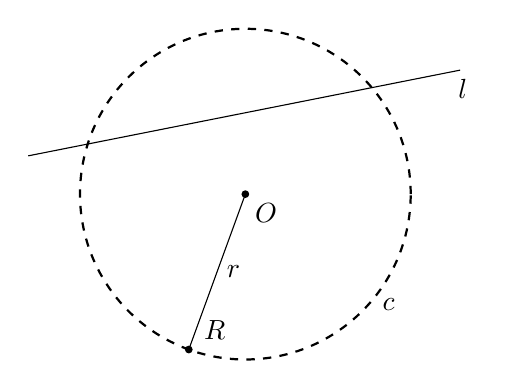
\begin{tikzpicture}[scale=.7]
\coordinate (O) at (0,0);
\node at (2.6,-2) {$c$};
\draw[thick,dashed] (O) circle[radius=3cm];
\fill (O) node[below right] {$O$} circle[radius=2pt];
\draw (O) -- node[right] {$r$} ++(-110:3cm) coordinate (R);
\fill (R) circle[radius=2pt] node[above right,xshift=2pt] {$R$};
\draw (O) +(170:4cm) -- node[below, near end,xshift=40pt,yshift=8pt] {$l$} ++(30:4.5cm);
\end{tikzpicture}
\vspace*{-8pt}
\end{center}
Let $2s$ be the length of chord $XY$, $M$ be its midpoint and $t$ be the distance $OM$.
\begin{quote}
\vspace*{-8pt}
By Prelim. 2, $M$ can be constructed as the intersection of the perpendicular from $O$ to line $l$. $X$, $Y$, $s$ are just definitions; we haven't constructed them yet.
\end{quote}
\begin{center}
\begin{tikzpicture}[scale=.7]
\coordinate (O) at (0,0);
\node at (2.6,-2) {$c$};
\draw[thick,dashed,name path=circle] (O) circle[radius=3cm];
\fill (O) node[below right] {$O$} circle[radius=2pt];
\draw (O) -- node[right] {$r$} ++(-110:3cm) coordinate (R);
\fill (R) node[above right,xshift=2pt] {$R$} circle[radius=2pt];
\draw[name path=l] (O) ++(170:4cm) -- node[below, near end,xshift=40pt,yshift=12pt] {$l$} ++(20:8cm);
\path[name intersections={of=circle and l,by={Y,X}}];
\fill (X) node[above left] {$X$} circle[radius=2pt];
\fill (Y) node[above right] {$Y$} circle[radius=2pt];
\draw[thick,dashed] (O) -- node[below] {$r$} (X);

\path (X) -- ($(X)!.5!(Y)$) coordinate (M);
\fill (M) node[above] {$M$} circle[radius=2pt];
\draw[thick,dashed] (O) -- node[right] {$t$} (M);
\path (X) -- node[above] {$s$} (M);
\path (M) -- node[above] {$s$} (Y);
\draw (O) ++(170:4cm) -- ++(20:3.1cm) -- ++(-70:10pt) -- ++(20:10pt);
\end{tikzpicture}
\vspace*{-6pt}
\end{center}
From right triangle $\triangle OMX$, $s^2=r^2-t^2$ or $s=\sqrt{(r+t)(r-t)}$ is constructible by Prelim 2, and $r \pm t$ by Prelim 3. $s$ can then be constructed by Prelim 5, and by Prelim 3 again, $X$ and $Y$ can be found. 
\begin{quote}
Define the length of $OM$ to be $t$. Prelim. 3 describes the construction of line segments of length $t$ from a point $O$ in the directions $OR$ and $RO$, thus constructing line segments of length $r\pm t$. Prelim. 5 describes the construction of a line segment of length $s=\sqrt{(r+t)(r-t)}$ and finally Prelim. 3 constructs line segments of length $s$ from point $M$ in both directions along line $l$, thus constructing the points $X$ and $Y$.
\end{quote}

\textbf{III.} \textit{Construct the points of intersection of two given circles.}

\textbf{Solution.} Let $c_1(O_1,r)$ and $c_2(O_2,r)$ be the two given circles, and $X$ and $Y$ be the points of intersection (to be constructed).
\begin{center}
\begin{tikzpicture}[scale=1.1]
\coordinate (O1) at (0,0);
\coordinate (O2) at (2.5,0);
\fill (O1) node[below left] {$O_1$} circle[radius=2pt];
\fill (O2) node[below right] {$O_2$} circle[radius=2pt];
\draw[thick,dashed,name path=circle1] (O1) circle[radius=2cm];
\draw[thick,dashed,name path=circle2] (O2) circle[radius=1.6cm];
\path [name intersections={of=circle1 and circle2,by={X,Y}}];
\draw (O1) -- node[above] {$r_1$} ++(160:2cm);
\draw (O2) -- node[above] {$r_2$} ++(30:1.6cm);
\fill (O1) ++(160:2cm) circle[radius=2pt];
\fill (O2) ++(30:1.6cm) circle[radius=2pt];
\draw (O1) -- (O2);
\node at (-1.7,1.6) {$c_1$};
\node at (3.8,1.4) {$c_2$};
\draw[<->] (0,-1) -- node[fill=white] {$t$} (2.5,-1);
\node at (6,0) {$t=O_1O_2$};
\end{tikzpicture}
\end{center}
% typos intersecton, resepectively
\begin{quote}
\vspace*{-8pt}
The circles are dashed to indicate that they haven't been constructed (and won't be constructed because we don't have a compass). $O_1,O_2$ are actual points so we can construct the line $O_1O_2$ with the straight-edge.
\vspace*{-12pt}
\end{quote}

Let $A$ be the point of intersection of $XY$ and the line of the centers $O_1O_2$.
\begin{quote}
\vspace*{-12pt}
Again, just definitions. $A,X,Y$ have not yet been constructed.
\vspace*{-12pt}
\end{quote}
Let $t$, $q$ and $x$ be the distances $O_1O_2$, $O_1A$ and $XA$ respectively.
\begin{center}
\begin{tikzpicture}[scale=1.1]
\coordinate (O1) at (0,0);
\coordinate (O2) at (2.5,0);
\fill (O1) node[below left] {$O_1$} circle[radius=2pt];
\fill (O2) node[below right] {$O_2$} circle[radius=2pt];
\draw[thick,dashed,name path=circle1] (O1) circle[radius=2cm];
\draw[thick,dashed,name path=circle2] (O2) circle[radius=1.6cm];
\path [name intersections={of=circle1 and circle2,by={X,Y}}];
\fill (X) node[above,yshift=4pt] {$X$} circle[radius=2pt];
\fill (Y) node[below,yshift=-4pt] {$Y$} circle[radius=2pt];
\draw[thick,dashed] (O1) -- node[above,xshift=-4pt] {$r_1$} (X);
\draw[thick,dashed] (O2) -- node[above,xshift=4pt] {$r_2$} (X);
\draw[name path=oo] (O1) -- (O2);
\node at (-1.7,1.6) {$c_1$};
\node at (3.8,1.4) {$c_2$};
\draw[name path=xy] (X) -- (Y);
\path[name intersections={of=xy and oo,by={A}}];
\fill (A) node[below left] {$A$} circle[radius=2pt];
\path (O1) -- node[below,xshift=-2pt] {$q$} (A);
\path (X) -- node[left,yshift=-2pt] {$x$} (A);
\draw[<->] (0,-1) -- node[fill=white] {$t$} (2.5,-1);
\node at (6,.5) {$t=O_1O_2$};
\node at (6,0) {$q=O_1A$};
\node at (6,-.5) {$x=XA$};
\end{tikzpicture}
\end{center}
We will show that $q$ and $x$ are constructible (in straight-edge geometry); then Prelim 3 will allow us to construct $A$ (at a distance of $q$ from $O_1$), Prelim 2 the perpendicular to $O_1O_2$ at $A$, and Prelim 3 $X$ and $Y$ (at a distance of $x$ from $A$) on this perpendicular.
\begin{quote}
\vspace*{-8pt}
$X$ and $Y$ are actually on the intersections of the circles since they are distances $r_1,r_2$ from $O_1,O_2$.
\vspace*{-8pt}
\end{quote}

\textbf{Finding q.} Apply the law of cosines to $\triangle O_1O_2X$ to get
\[
\renewcommand*{\arraystretch}{1.8}
\begin{array}{rcl}
r_2^2 &=& r_1^2 + t^2 - 2r_1t\cos\angle XO_1O_2\\
      &=& r_1^2 + t^2 - 2t(r_1\cos\angle XO_1O_2)\\
&=& r_1^2 + t^2 - 2tq\\
2tq &=& (r_1^2+t^2) - r_2^2\,.
\end{array}
\]
Set $d=\sqrt{r_1^2+t^2}$ so that $q=\frac{(d+r_2)(d-r_2)}{2t}$. $d$, the hypotenuse of a right triangle with legs of length $r_1$ and $t$, is constructible by Prelims 2 and 3, $n= d+ r_2$, $m= 2t$, $s =d -r_2$ are constructible by Prelim 3, and $q=\frac{n}{m}s$ is constructible by Prelim 4.
\begin{quote}
\vspace*{-8pt}
The right triangle with sides $d,r_1,t$ doesn't appear in the above diagram. We construct it somewhere in the plane for the purpose of computing $d$ from the given lengths $r_1,t$ and then $q$ from $d,r_2,t$. 
\vspace*{-8pt}
\end{quote}
\textbf{Finding x.} From (right) $\triangle AO_1X$, $x^2=r_1^2-q^2$, and $x=\sqrt{(r_1+q)(r_1-q)}$. Prelim 3 provides a construction of $h =r_1+ q$ and $k= r_1 - q$, and Prelim 5 a construction of $x= \sqrt{hk}$. 

